\documentclass[../chapter-2-spline-representation.tex]{subfiles}
\begin{document}
We equip the $l$ and $m$ axes each with a B-spline basis to construct a basis for the varying coefficient function $\phi$ in \ref{eq:phi-star} by taking the tensor product of the two marginal bases. Let 
\[
B_{1}\left(l\right),\dots, B_{K}\left(l\right)  \mbox{ and } B_{1}\left(m\right),\dots, B_{L}\left(m\right)
\]
denote the B-spline bases for $l$ and $m$, each having a set of equally spaced knots along their respective domain. It is worth noting that while we have chosen not to distinguish between $\left\{ B_k \right\}$ and $\left\{ {B}_l \right\}$ for the sake of brevity, one is free to specify a different basis for each dimension either by using different order B-spline or, of course, using different numbers of knots, and hence entirely different knot sequences since P-splines rely on bases with equally spaced knots. The tensor product basis functions
\begin{equation*}
T_{jk}\left(l,m\right) = B_j\left(l\right){B}_k\left(m\right)
\end{equation*}
\noindent
carve the $l$-$m$ domain into rectangles.  Figure~\ref{fig:sparse_bicubic_BS_basis} shows a thinned tensor product basis $\left\{ T_{kl} \right\}$; a portion of the basis was omitted to eliminate overlapping of the basis functions so that the reader can identify individual tensor products. Each ``hill'' in Figure~\ref{fig:sparse_bicubic_BS_basis} is associated with an unknown coefficient $\theta_{ij}$ which determines the height of the hill. For a given knot grid, we can approximate a surface by

\begin{equation} \label{eq:varying-coefficient-tensor-product-expansion}
\phi\left(l,m\right) = \sum_{i=1}^K \sum_{j=1}^L \theta_{ij} B_{i}\left(l\right) B_{j}\left(m\right), 
\end{equation}
\noindent
and the function evaluated at the observed $\left(l_{ijk}, m_{ijk}\right)$ may be written 
\begin{equation*} 
\vphistar = B_m \Theta B_l^\prime
\end{equation*}
\noindent 
where $\Theta$ denotes the $K \times L$ matrix of tensor product coefficients, with elements $\theta_{ij}$.

\begin{figure}[H]
\centering
 \graphicspath{{img/}}
  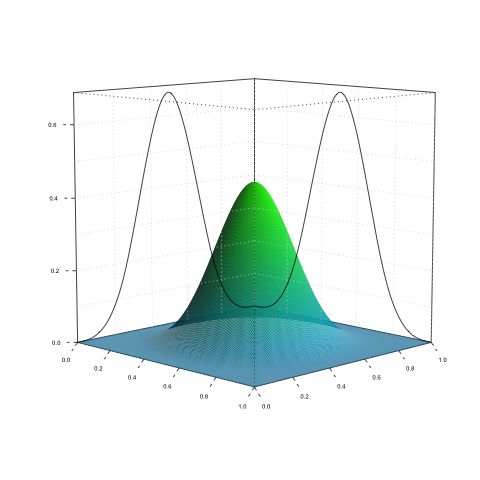
\includegraphics[width=4in, height=4in]{bicubic_basis_function.png}
 
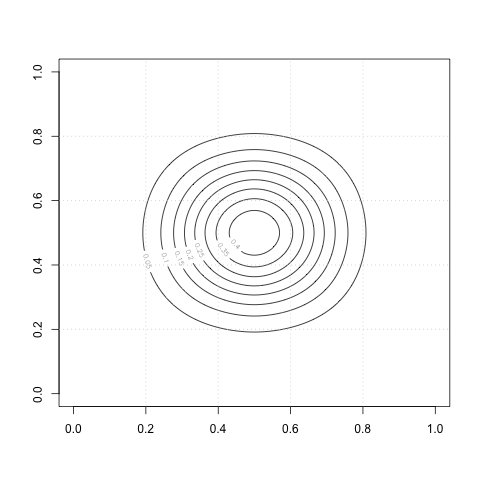
\includegraphics[width=4in, height=4in]{bicubic_bspline_contour.png}
\caption{Tensor product of two cubic B-splines}
\label{fig:bicubic_BS}
\end{figure}

\begin{figure}[H]
  \centering
  \graphicspath{{img/}}
  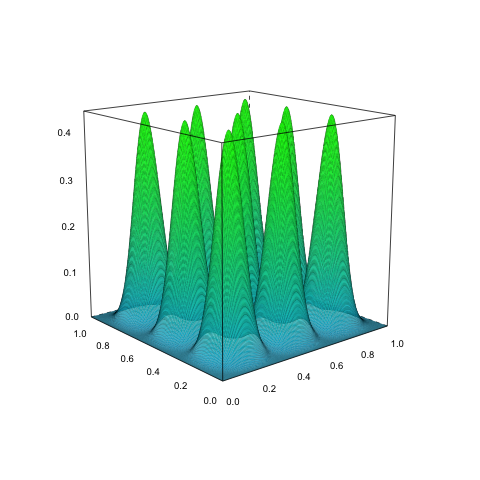
\includegraphics[width=5in,height=5in]{sparse_bicubic_basis.png}
  \caption{A subset of a full bivariate basis of cubic B-splines}\label{fig:sparse_bicubic_BS_basis}
\end{figure}

\subsection{Regularization with difference penalties} \label{subsection:univariate-psplines}

The minimizer of \ref{eq:loglikelihood} honors the fidelity to the data, so to balance the complexity of the fitted function with the goodness of fit to the data, we can append a penalty to the negative log likelihood to control the fitted function. By using rich B-spline bases for $l$ and $m$ alongside discrete difference penalties on the spline coefficients, we can achieve as much smoothness of the fitted function in both the $l$ and $m$ dimensions as desired. \citet{o1986statistical} was the first to propose using a rich B-spline basis and using a penalty to restrict the flexibility of the fitted curve, like \citet{wahba1990spline} applying a penalty to the second derivative of the fitted curve:
\[
J = \int_0^1 \left[ f^{\prime \prime}\left(l\right)\right]^2\;dx.
\]

For a B-spline of the form
\[
f\left(x\right) = \sum\limits_{j=1}^n \theta_i B_j\left(x\right),
\]
one can derive a banded matrix $P$ using the properties of B-splines such that 
 \[
 J = \theta^\prime P \theta
 \] 
 \noindent
 where $\theta = \left(\theta_1,\dots, \theta_n\right)$. The $i$-$j^{th}$ element of $P$ is given by
 \[
 p_{ij} = \int_0^1 B_i^{\prime \prime} \left( x \right)B_j^{\prime \prime} \left( x \right)\;dx.
 \]

%As discussed in Section 2, we can define an entire class of functional autoregressive models using only the $l$ direction, and additionally, as discussed in Section 3, there is a natural expectation about the functional form of the autoregressive coefficient function (and hence covariance) as a function of $l$. The use of smoothing splines to estimate $\phi$ outlined in Section~\ref{} yields smooth null models, but smoothness of the elements of the Cholesky factor alone may not lead to desirable structure in the inverse covariance matrix.  

%
%These approaches implicitly adopt different notions of sparsity. Like \citet{huang2006covariance} and \citet{levina2008sparse}, our aim is to regularize the inverse of the covariance matrix through the Cholesky factor. Expressing the varying coefficient function using a tensor product basis expansion builds the foundation for a flexible estimation framework within which employing multiple notions of smoothness is simple and straightforward. 
%

In some applications, it is useful to work with third and fourth order differences, since for large values of $\lambda$, the fitted curve approaches a parametric polynomial model. This may be of particular interest in the context of estimating the elements of the Cholesky factor, as many have proposed simple parametric functions of lag only for $\phi$, such as low order polynomials. See \citet{pourahmadi1999joint}. However, with the use of higher order derivatives, the computation of $P$ is nontrivial and becomes very tedious. \citet{eilers1996flexible} were the first to propose P-splines, or \emph{penalized B-splines}, as an approach to nonparametric regression. P-splines circumvent complexity associated with constructing such penalty matrices by omitting derivatives and integrals altogether, replacing them with finite differences and sums. 

Instead, flexibility of the fitted function is controlled by using a discrete penalty matrix based on finite difference formulas. Smoothness of the fitted function is achieved by first using a rich B-spline basis with equally spaced knots to purposefully overfit the smooth coefficient vectors; this eliminates the difficulty of choosing the optimal set of knots. Then by attaching a difference penalty to the goodness of fit measure, one may prevent overfitting and make a potentially ill-conditioned fitting procedure a well-conditioned one. The finite difference penalty is simple to compute and can be handled mechanically for any order of the differences. Since it is easily introduced into regression equations, it is feasible to evaluate the impact of different orders of the differences on the fitted model.  Using the properties of B-splines, it is straightforward to show that the difference penalty of order $d$ is a good discrete approximation to the integrated square of the $d^{th}$ derivative, so little is lost by replacing the derivative-based penalty with

\begin{equation} \label{eq:bspline-difference-penalty}
J_d\left( f \right) = \sum_{j=d}^n \left(\Delta^d \theta_j\right)^2
\end{equation} 
\noindent
where $\theta = \left( \theta_1,\dots,\theta_n \right)$. Let $D_d$ denote the matrix difference operator: $D_d\theta = \Delta^d \theta$, where

 \begin{align*}
 \Delta \theta_j &= \theta_j - \theta_{j-1}, \quad  \Delta^2 \theta_j = \Delta\left(\Delta \theta_j\right) = \theta_j - 2\theta_{j-1} + \theta_{j-2}
 \end{align*}
\noindent 
In general,
\begin{equation*}
\Delta^d \theta_j = \Delta\left(\Delta^{d-1} \theta_j \right).
\end{equation*} 
\noindent
Then, \ref{eq:bspline-difference-penalty} can be written in terms of the squared norm of the difference operator applied to the vector of B-spline coefficients:
\begin{align} 
\begin{split} \label{eq:bspline-difference-penalty-vector-form}
J_d\left( f \right) &= \vert \vert D_d\theta \vert \vert^2 \\
&= \theta^\prime P_d \theta
\end{split}
\end{align}
\noindent
where $P_d = D_d^\prime D_d$.  To examine the connection between the second-derivative penalty to the penalty on second-order differences of the B-spline coefficients, we only need to employ straightforward calculus and exploit the recursive property of the B-spline basis functions:

\begin{equation*} 
\int_0^1 \left[ f^{\prime \prime}\left(x\right)\right]^2\;dx = \int_{0}^{1} \left\{ \sum\limits_{j=1}^n  \theta_j B_{j,3}^{\prime \prime} \left(l\right) \right\}^2\; dl.
\end{equation*}
\noindent
The derivative properties of B-splines permits this to be written as 
\begin{equation*} \label{eq:second-derivative-bspline-penalty}
\int_0^1 \left[ f^{\prime \prime}\left(x\right)\right]^2\;dx =  \int_{0}^{1}  \bigg[ \sum\limits_{j=1}^n \sum\limits_{k=1}^n \Delta^2 \theta_j \Delta^2 \theta_k B_{j,1}\left(l\right)B_{k,1}\left(l\right)\bigg]\; dl  . 
\end{equation*}
\noindent
Most of the cross products of $B_{j,1}\left(x\right)$ and $B_{k,1}\left( x \right)$ vanish since B-splines of degree 1 only overlap when $j$ is $k-1$, $k$, or $k+1$. Thus, we have that
\begin{align}
\begin{split}
\int_0^1 \left[ f^{\prime \prime}\left(x\right)\right]^2\;dx  = {} &  \int_0^1 \bigg[ \left\{ \sum\limits_{j=1}^n   \Delta^2 \theta_j  B_j\left(l,1\right)  \right\}^2  + 2 \sum_{j}\Delta^2 \theta_j\Delta^2 \theta_{j-1}B_j\left(l,1\right)B_{j-1}\left(l,1\right) \bigg]\; dl \\ 
= {} & \sum \limits_{j=1}^n  \left( \Delta^2\theta_j \right)^2 \int_0^1 B_j^2\left(l,1\right)\;dl \\
   &{} \;\;\;\;\;\;\;\;\;\;\;\;\;\;\;\;\;\; + 2 \sum\limits_{j=1}^n \Delta^2 \theta_j\Delta^2 \theta_{j-1} \int_0^1 B_j\left(l,1\right)B_{j-1}\left(l,1\right)\;dl 
\end{split}
\end{align}
\noindent
which can be written as
\begin{equation} \label{eq:derivative-penalty-difference-penalty-connection}
\int_0^1 \left[ f^{\prime \prime}\left(x\right)\right]^2\;dx  = c_1 \sum\limits_{j=2}^n \left( \Delta^2 \theta_j\right)^2 + c_2 \sum\limits_{j=3}^n \Delta^2 \theta_j\Delta^2 \theta_{j-1}
\end{equation}
\noindent
Given a set of equidistant knots, the constants $c_1$ and $c_2$ are given by
\begin{equation}
\begin{split}
c_1 & =   \int_0^1 B_{j,1}^2\left(x\right) dx\\
c_2 & = \int_0^1 B_{j,1}\left(x\right)B_{j-1,1}\left(x\right) dx.
\end{split}
\end{equation}

This gives us that the traditional smoothness penalty on the squared second derivative can be written as a linear combination of a penalty on the second-order differences of the B-spline coefficients \ref{eq:bspline-difference-penalty} and the sum of the cross products of neighboring second differences. The second term in \ref{eq:derivative-penalty-difference-penalty-connection} leads to a complex objective function when minimizing the penalized likelihood, where seven adjacent spline coefficients occur, as opposed to five if only the first term in \ref{eq:derivative-penalty-difference-penalty-connection} is used in the penalty. The added complexity is a consequence of overlapping B-splines, which quickly increases when using higher order differences and higher order B-splines. We can seamlessly augment the likelihood with the difference penalty to achieve smooth fitted functions without the complexity posed by the derivative-based penalty.
%citet{chen2011efficient}, citet{pourahmadi1999joint}, and citet{pourahmadi2002dynamic} have elicited parametric models for the generalized autoregressive coefficients, letting the GARPs depend only on the distance between two time points.

A smoother sequence of coefficients leads to a smoother curve, as illustrated in Figure~\ref{fig:second_ord_PS_pen_SML_lambda}.  The relationship between P-spline curves and their coefficients is easily characterized if we consider the coefficients as the skeleton of the function, and draping the B-splines over them puts the flesh on the bones. As long as the coefficient sequence is smooth, the number of basis functions (and coefficients) is unimportant since the penalty ensures the smoothness of the skeleton and that the fitting procedure is well-conditioned. Figure~\ref{fig:overcomplete_basis_pspline} illustrates this utility of the penalty for simulated data; there are $m=10$ observations and $60$ cubic B-splines. This property of P-splines cannot be overly appreciated because it frees us from the concern of choosing the optimal set of knots. Unless computational constraints are of concern, which is possible with large models, it is prudent to use even more B-splines. Figure~\ref{fig:PS_penalty_section_figure_2} shows how the fitted function changes as the tuning parameter varies when the data are sparsely sampled. P-splines enjoy a number of additional advantageous properties, many of which are inherited from the attractive properties of B-splines. See \citet{eilers1996flexible}  for a detailed presentation. 

\begin{figure}[H] \label{fig:PS-smoothing-figure-1}
\begin{subfigure}{.5\textwidth}
  \centering
   \graphicspath{{img/}}
  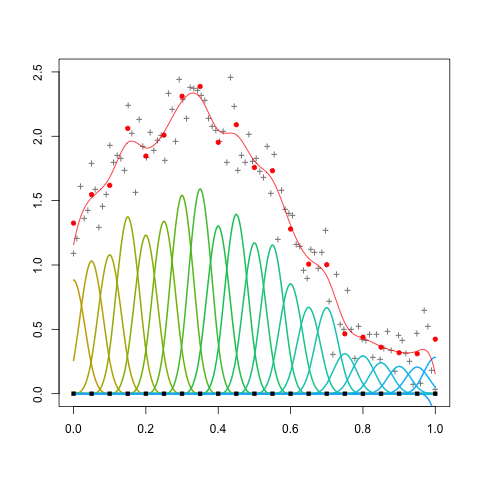
\includegraphics[scale=0.5]{pspline_pord2_xsmall_lambda.png}
  \label{fig:pspline_small_lambda}
\end{subfigure}
\begin{subfigure}{.5\textwidth}
  \centering
   \graphicspath{{img/}}
  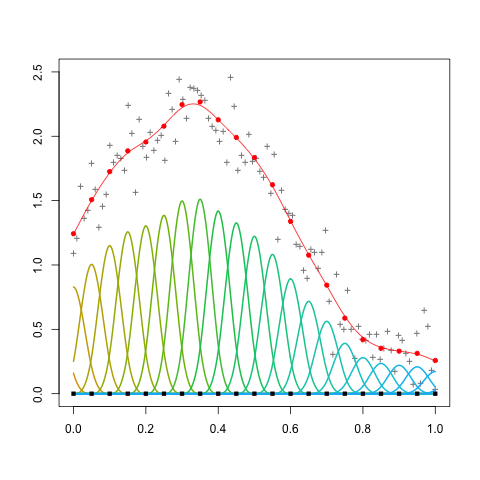
\includegraphics[scale=0.5]{pspline_pord2_small_lambda.png}
  \label{fig:pspline_small_lambda}
\end{subfigure}
\begin{subfigure}{.5\textwidth}
  \centering
   \graphicspath{{img/}}
  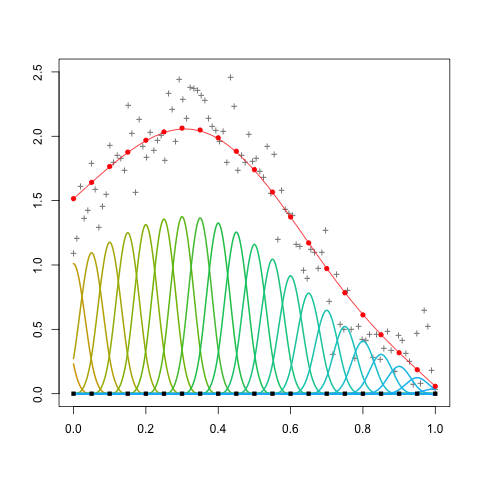
\includegraphics[scale=0.5]{pspline_pord2_medium_lambda.png}
  \label{fig:pspline_small_lambda}
\end{subfigure}
\begin{subfigure}{.5\textwidth}
  \centering
   \graphicspath{{img/}}
  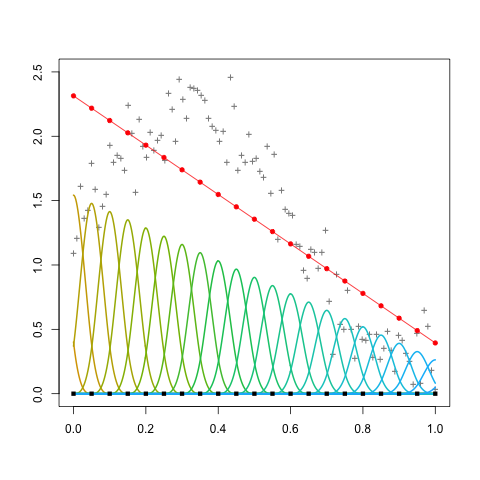
\includegraphics[scale=0.5]{pspline_pord2_large_lambda.png}
  \label{fig:pspline_small_lambda}
\end{subfigure}
\caption{\textit{Illustration of the impact of the second order difference penalty. The number of B-splines used is the same in each plot, with the value of the penalty parameter increasing from left to right and top to bottom across each plot. The fitted curve in the upper left plot is the most ``wiggly'' of any of the fits, as the penalty plays the weakest roll in the fitted coefficients there. The red circles are the values of each of the B-spline coefficients; as the penalty increases, they form as smoother sequence as we move across the four plots, which results in a smoother fitted function. As the penalty parameter approaches infinity, the fit approaches a linear function as shown in the bottom right plot.}}
\label{fig:second-ord-PS-pen-SML-lambda}
\end{figure}


%First, unlike many types of kernel smoothers, P-splines show no boundary effects i.e. the spreading of the fitted curve outside of the physical domain of the data, usually while also bending toward zero. See \citet{eilers1996flexible} Section 8 for a detailed discussion.

%P-splines can fit polynomial data exactly. Given data $\left(l_i,y_i\right)$, if the $y_i$ are a polynomial in $l$ of degree $k$, then B-splines of degree $k$ or higher will fit the data exactly.  The same is true for P-splines if the order of the penalty is $k+1$ or higher, irrespective of the value of $\lambda$. An informal proof is left to the appendix.
%
%Under a difference penalty of order $k$, the fitted function will approach a polynomial of degree $k-1$ for large values of $\lambda$ as long as the degree of the B-splines is greater than or equal to $k$. This can be shown by once again considering the relationship between the derivatives of a B-spline fit and the differences in neighboring coefficients; detailed discussion is left to the appendix. Figure~\ref{fig:PS_penalty_section_figure_6} visually demonstrates this property by examining the behavior of the fitted function as the tuning parameter varies under a difference penalty of order $d=0,1,2,3$.
%
%We will leverage several properties of the smoothing matrix, $H$, for model evaluation and selection, so focus on the linearized smoothing problem solved at each value of the penalty parameter, $\lambda$, is prudent. The trace of $H$ approaches the order of the differencing operator, $k$ for larges values of $\lambda$. The trace of the smoothing matrix is a useful measure of effective model dimension, so understanding its limiting behavior is important. 



To extend these results to the bivariate setting for regularizing of $\phi$, the only modification to the differencing procedure in one dimension necessary is the addition of a second difference penalty, one for each variable $l$ and $m$. We append the pair of penalties to the negative log likelihood \ref{eq:loglikelihood} and take the estimator of $\phi$ to correspond to the B-spline coefficients minimizing

\begin{align} 
\begin{split}\label{eq:unfolded-difference-penalty-log-likelihood}
-2L + J\left(\phi\right) = \sum_{i=1}^N \sum_{j=2}^{m_i} \sigma\left({t_j}\right)^{-2} \left\{y_{ij} - \sum_{k=1}^{j-1} \left( \sum_{r=1}^L \sum_{s=1}^K \theta_{rs} B_r\left(l_{ijk}\right)B_s\left(m_{ijk}\right)\right)y_{ik} \right\}^2 \\ 
+ \lambda_l \sum_{r^\prime=1}^K \vert D_{d_{\ms l}} \theta_{r^\prime \cdot} \vert^2 + \lambda_m \sum_{s^\prime=1}^L \vert D_{d_{\ms m}} \theta_{\cdot s^\prime} \vert^2.
\end{split}
\end{align}


%\begin{align*}\label{eq:unfolded-row-column-difference-penalty}
%\mathcal{Q}=\sum_{i=1}^n \sum_{j=2}^{m_i} \sigma_{ij}^{-2} \left[y_{ij} - \sum_{k=1}^{j-1}\left(\sum_{i=1}^K \sum_{j=1}^L \theta_{ij} B_{i}\left(l_{ijk}\right) B_{j}\left( m_{ijk} \right)  \right) y_{ik} \right]^2 \\
%\mbox{\;\;\;\;\;\;\;\;}+ \lambda_l \sum_{k} \vert D_d \theta_{k \cdot} \vert^2 + \lambda_m \sum_{l} \vert D_{\ms d_{\ms m}} \theta_{\cdot l} \vert^2 
%\end{align*}

\noindent
where $\theta_{k \cdot}$ and $\theta_{\cdot l}$ denote the $k^{th}$ row and $l^{th}$ column of $\Theta$, respectively. The first term in\ref{eq:unfolded-row-column-difference-penalty} imposes a difference penalty of order $d_{\ms l}$ on the rows of the coefficient matrix while the second term places a difference penalty (of possible different order $d_{\ms m}$) on the columns. We give each direction its own smoothing parameter to permit anisotropic smoothing; however, one could opt to use a single smoothing parameter for both directions and dodge the added work of optimizing the amount of smoothing with two separate parameters. Figure ~\ref{fig:2d_PS_penalty_demo} shows a potential result of heavy column penalization (left) and heavy row penalization (right) under a second order difference penalty on each row and each column for large values of $\lambda_l$ and $\lambda_m$. The figure demonstrates that the limiting behaviour of each row and column is linear, but the resulting surface may exhibit slope reversals from one row (column) to the next. 


\begin{figure}[H] \label{fig:2d_PS_penalty_demo}
 \begin{subfigure}{.48\textwidth}
  \centering
   \graphicspath{{img/}}
 \includegraphics[scale=0.5]{"model selection/effective dimension/2d_PS_section_figure1_big_col_lambda"}
 \caption{\textit{heavy column penalty}}
 \label{fig:2D_PS_big_col_penalty}
 \end{subfigure}
 \begin{subfigure}{.48\textwidth}
  \centering
   \graphicspath{{img/}}
  \includegraphics[scale=0.5]{"model selection/effective dimension/2d_PS_section_figure1_big_row_lambda"}
 \caption{\textit{heavy row penalty}}
\label{fig:2D_PS_big_row_penalty}
 \end{subfigure}
 \caption{\textit{Nine cubic B-spline tensor products with heavy linear column penalty and heavy linear row penalty}}
\end{figure}
\noindent
We take the estimator of $\phi$ to be the minimizer of 
It is computationally advantageous to express the coefficient matrix in ``unfolded'' notation, which allows us to express the varying coefficient function at the observed coordinate grid as in the usual multiple regression form:

\begin{equation*}
\mbox{vec}\left\{\phi\left(l,m\right)\right\} = B \theta
\end{equation*}
\noindent
Stacking the columns of $\Theta$ gives the vectorized coefficient matrix $\theta = \mbox{vec}\left( \Theta \right)$. The $p \times KL$ tensor product basis $B$ is constructed from the tensor product of the marginal B-spline bases defined in \citet{eilers2006fast} as the \textit{row-wise Kronecker product} of the individual bases:

\begin{equation} \label{eq:rowwise-kronecker-product}
B = B_l \square B_m = \left( B_m \otimes 1^\prime_{K} \right) \odot \left(1^\prime_{L} \otimes  B_l  \right).
\end{equation}
\noindent
The operator $\odot$ denotes the element-wise matrix product; $1_K$ ($1_L$) denotes the column vector of ones having length $K$ ($L$.) The operations in \ref{eq:rowwise-kronecker-product} construct $B$ such that the $i^{th}$ row of $B_m\square B_l$ is the Kronecker product of the corresponding rows of $B_m$ and $B_l$. The penalty in \ref{eq:unfolded-row-column-difference-penalty} can also be compactly expressed:

\begin{equation*} \label{eq:tensor-product-penalty}
\lambda_l \vert \vert P_l \theta \vert \vert^2 + \lambda_m \vert \vert P_m \theta \vert\vert^2
\end{equation*}

where $P_l = I_L \otimes D_{d_{\ms l}}^\prime D_{d_{\ms l}} $ and $P_m =  D_{d_{\ms m}}^\prime D_{d_{\ms m}} \otimes I_K$. We define the matrix $W$ of historical regressors so that \ref{eq:unfolded-difference-penalty-log-likelihood} can be written in matrix form as

\begin{equation} \label{eq:tensor-pspline-objective-function}
-2L + J\left(\phi\right) = \left( Y - WB\theta\right)^\prime D^{-1}\left( Y - WB\theta\right)  + \lambda_l \vert\vert P_l \theta \vert\vert^2 + \lambda_m \vert\vert P_m \theta\vert \vert^2,
\end{equation}
\noindent
with $\hat{\theta}$ solving the system of equations 
\begin{equation} \label{eq:tensor-pspline-normal-equations}
\left[ \left(WB\right)^\prime D^{-1} WB +  \lambda_l P_l+ \lambda_m P_m\right]\theta = \left(W B\right)^\prime D^{-1}Y
\end{equation}
\noindent
From \ref{eq:tensor-pspline-normal-equations}, we note that the system of equations depends on basis coefficients remains fixed at $KL$, even as the number of observations increases.   The grid of regression coefficients can be recovered by arranging the elements of $\hat{\theta}$ into a matrix of $L$ columns having length $K$. 

This recipe for constructing a tensor product basis for $\phi$ is an easy and convenient way to construct a two-dimensional basis for a bivariate function with domain corresponding to the unit square. However, the domain of the autoregressive coefficient function, specified in \ref{eq:phi-star-domain}, lies on the lower triangle of the unit square:

\begin{figure}[H] \label{fig:triangle-domain}
    \graphicspath{{img/}}
 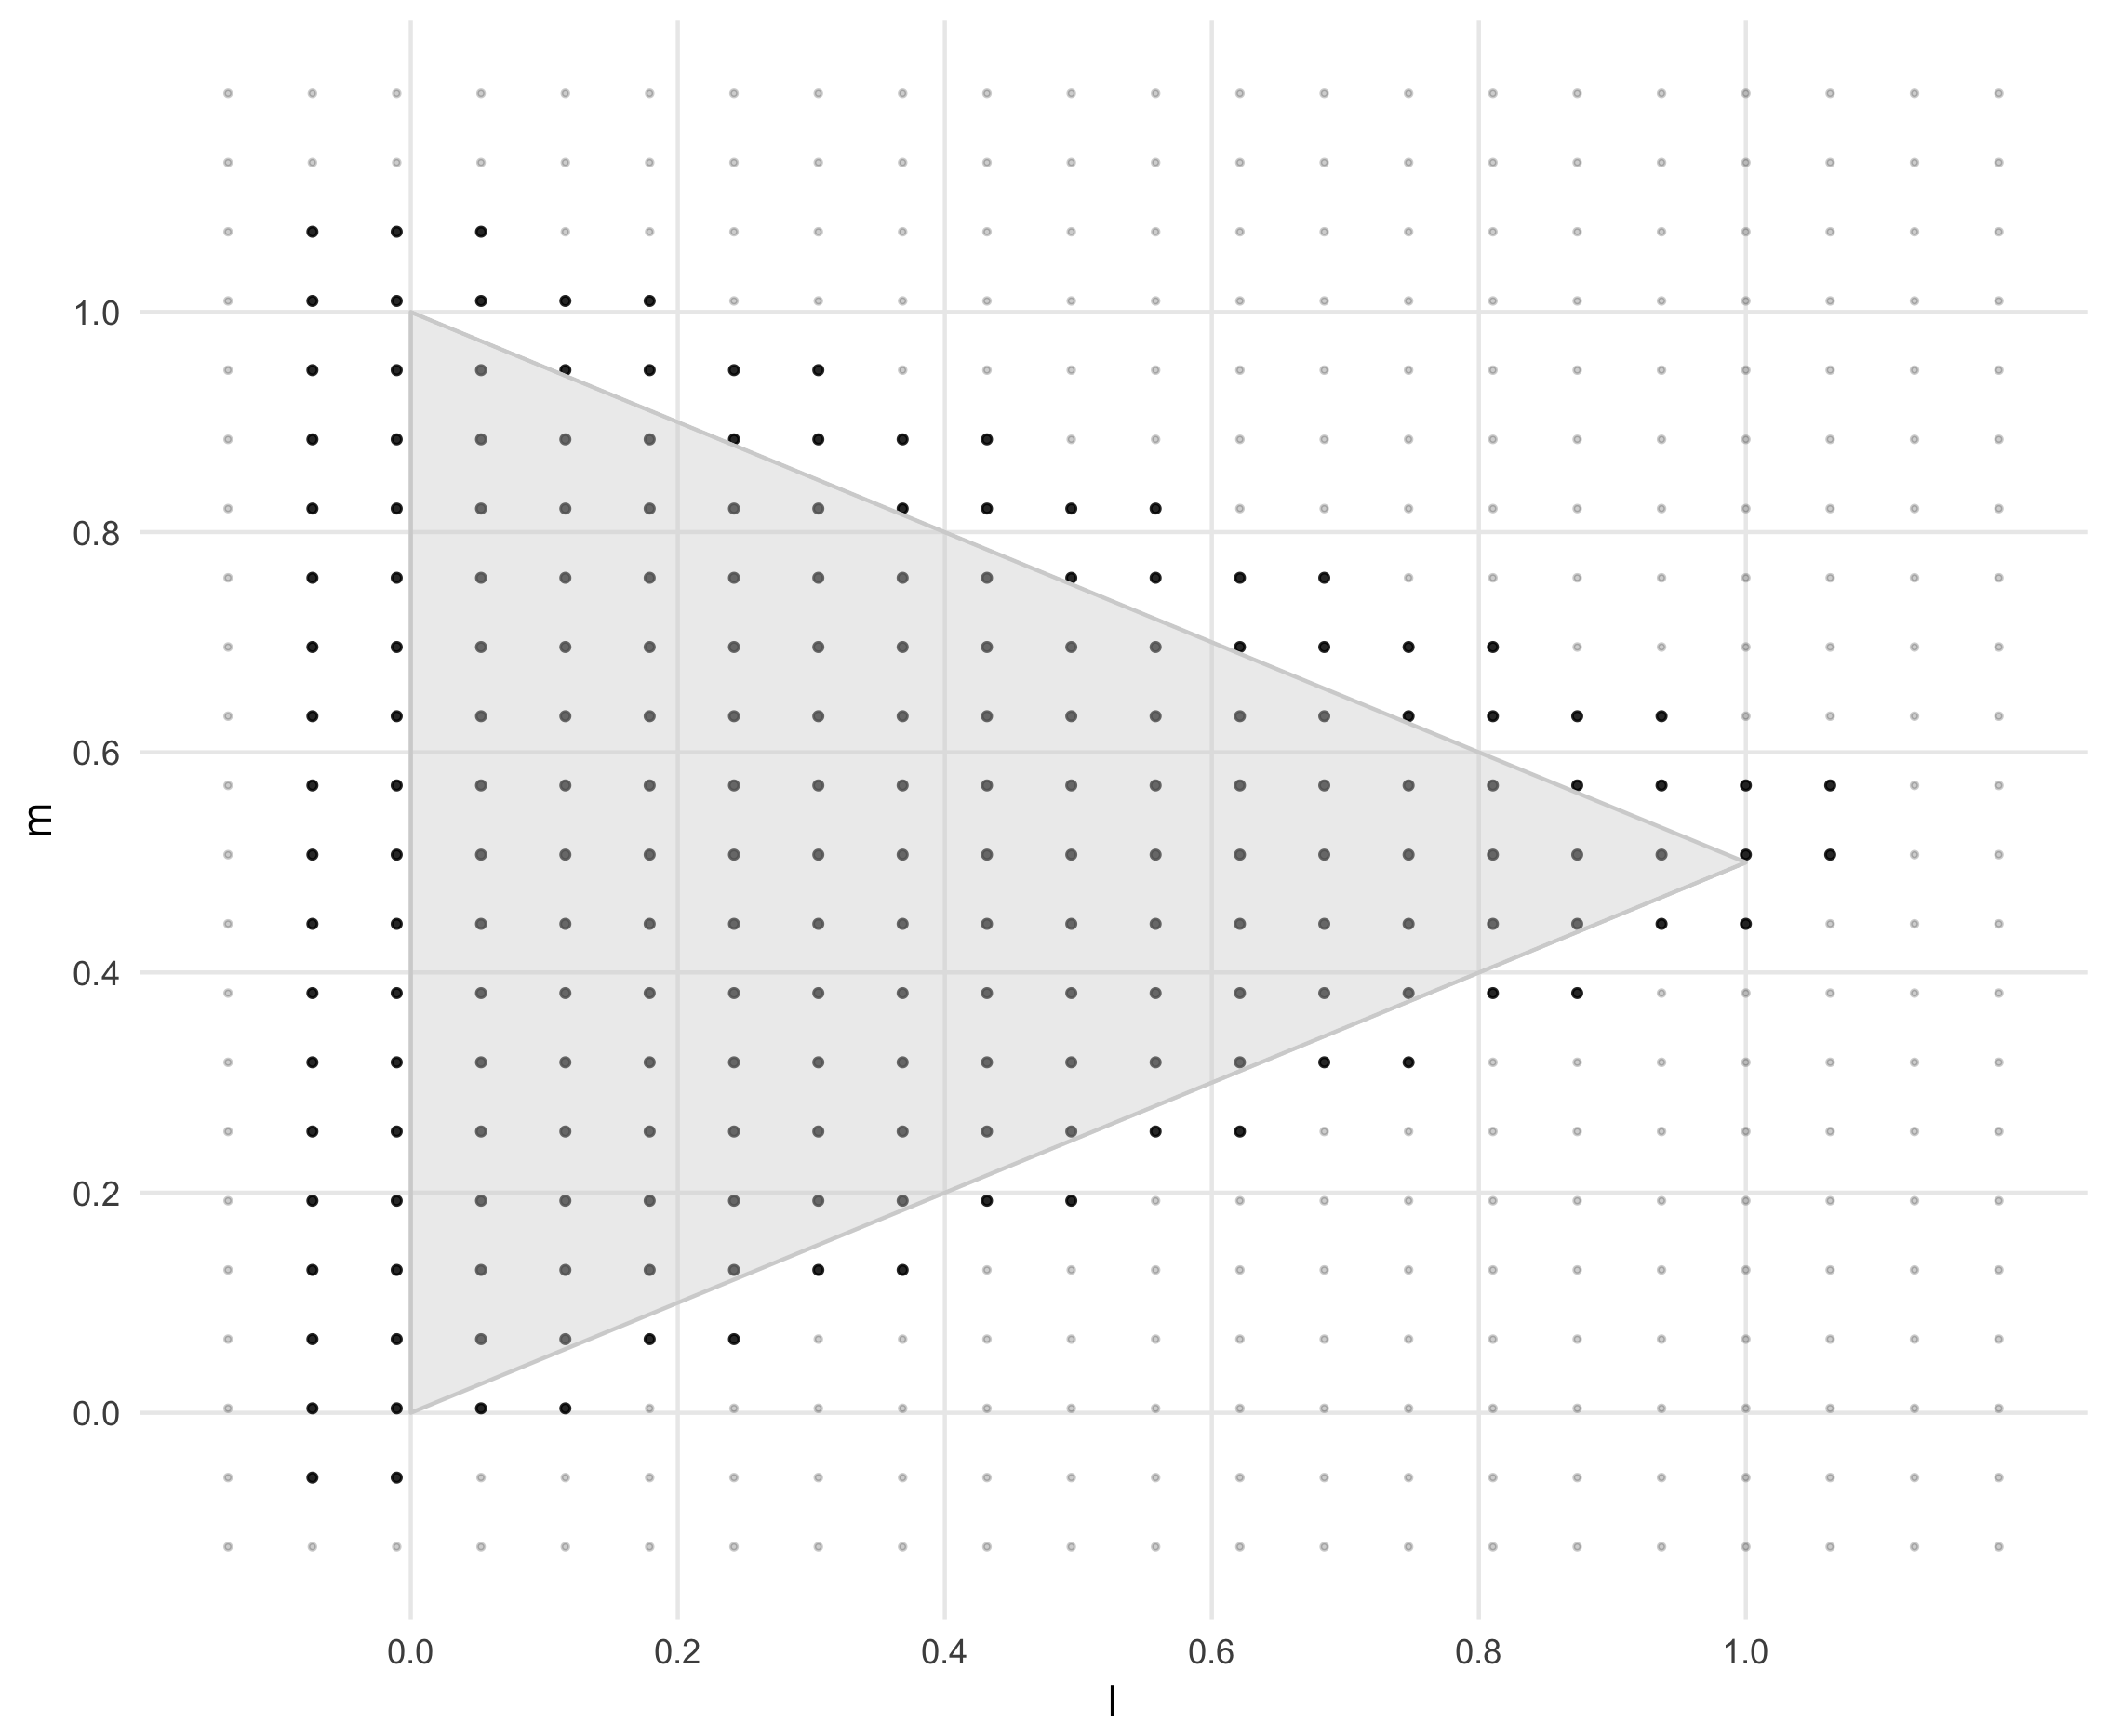
\includegraphics[scale=0.2]{knot-removal-on-triangle-domain.png}
 \caption{$\frac{l}{2} < m < 1 - \frac{l}{2}, \quad 0 < l < 1.$}
 \end{figure}

The triangular domain of $\phi$ cannot be modeled by the tensor product basis as constructed due to singularities resulting from the large number of basis functions anchored at knots near which we have no data, and hence little information about the corresponding basis coefficient. Much work in computer graphics has been done proposing methods of smoothing over arbitrary function domains, which are approximated by triangulations. See \citet{dahmen1992blossoming} and \citet{seidel1991symmetric} for details. These methods are, however, quite computationally intensive; to correct for the instability in the smoothed surface, we can simply remove the knots corresponding to tensor products functions which do not overlap with the function domain from the basis, $B$, and trimming the penalty matrices $P_l$ and $P_m$ as needed. With the trimmed basis and penalties, we can carry out optimization as previously discussed.
\end{document}
